\documentclass{article}
\usepackage{graphicx}
\usepackage{amssymb}
\usepackage{amsmath}
\usepackage{tikz}
\usepackage{url}
\usepackage{color}
\usepackage{savetrees}
\usepackage{listings}
\usetikzlibrary{shapes}


\linespread{1.5}
\setlength{\parindent}{0pt}
\setlength{\parskip}{1.9ex plus 0.5ex minus 0.2ex}

\title{CSE638 \\ Advanced Graduate Algorithms (and Data Structures) -- Homework-3}

\author{Dhruv Matani (108267786) \& Gaurav Menghani (108266803)}

\begin{document}
\maketitle

\clearpage

\tableofcontents

\clearpage

\section{Summary of Weight Balance}

\subsection{Weight Balanced Search Tree}

\subsubsection{Search cost: $O(\log{n})$}

Since the tree is \textit{weight balanced}, the number of nodes in the
left subtree is a constant fraction away from the number of nodes in
the right subtree. This means that the tree is also height balanced
(i.e. the height of the left and right subtrees are within constant
fractions of each other).

Hence, any root to leaf path in such a tree will not touch more than
$O(\log{n})$ nodes.

\subsubsection{Worst case update cost: $O(\log{n})$}

To update such a structure, we use \textit{tree rotations}. The
rotations are similar to the \textit{AVL Tree Rotations} we perform to
balance an AVL Tree.

On an insert, we check if the balance conditions are met. If they are,
we don't perform any rotations, and move up to the parent root and
check the balance at the parent node.

Once we find a node that is out of balance, we need to perform either
a single left (or right) rotation or 2 rotations in succession. The 2
cases we need to handle (which are symmetric) are:

\begin{enumerate}
\item If the right child is heavier than the left child and the left
  child of the right child of the imbalanced node is heavier than its
  right sibling, we perform a right rotation around the right child of
  the current node followed by a left rotation around the current
  node.

\item If the right child is heavier than the left child and the left
  child of the right child of the imbalanced node is NOT heavier than its
  right sibling, we perform a single left rotation around the current
  node.

\end{enumerate}

\subsubsection{Amortized update cost: $O(\log{n})$ (rebalance whole subtree below a node)}

To rebalance a node by re-creating the subtree under it, we perform an
$O(n)$ operation to find the median of the subtree to be re-written
and make the subtree as balanced as possible. The cost to update a
subtree is therefore:

Cost to update =
$\dfrac{\#\ of\ nodes\ to\ rewrite}{\#\ of\ nodes\ that\ caused\ subtree\ to\ go\ out\ of\ balance}$

$=\dfrac{\Theta(n)}{\Omega(n)} = O(1)$

However, since updating a node causes all the subtreed along the
root-to-leaf path of which it is a part to go out of balance, we
charge this node $\Theta(\log{n}) * O(1)$ per update
$=\Theta(\log{n})$.

% External Memory Problems

\section{External Sorting}

We have $N$ elements and $B$ is the number of numbers in a
block. Hence, we have $\frac{N}{B}$ blocks.\\ Let $X =
\frac{N}{B}$. Also, let the number of blocks that we can fit in main
memory be $Y = \frac{M}{B}$.
\\
Since we are only interested in the number of blocks being
transferred, we don't worry about the actual computational complexity
of performing the sort (or merge).\\

\subsection{Algorithm Description}

\begin{enumerate}
\item We start off by assuming the input to be $X$ blocks of
  integers. We only deal in number of blocks from now.
\item We start off with $X$ \textit{runs} which contain $1$ block
  each.
\item Read in $Y$ blocks of input and merge them
  \textit{in-place}. We store metadata about each sequence's end so
  that we know when we run out of numbers in a block.
\item Once we run out of numbers in a block, we shall read off one more
  block from the same \textit{run} from which this block
  originated. If no more blocks exist in this run, we do nothing and
  wait for some other block to become empty.
\item As soon as a block becomes empty, we write it out to
  disk. Continuous write like this will result in a sorted sequence of
  blocks that are $Y$ more in ratio than the number of blocks in the
  input. For example, if we have $Y = 4$ and we start off with $32$
  runs of size $1$ block each, then we land up with $8$ runs of size
  $4$ blocks each after the first round, $2$ runs of size $16$ after
  the second round, and so on \ldots{}
\item Once we completely exhaust all blocks in a run, we then start
  processing the next set of $Y$ runs.
\item It is easy to see that we are reducing the number of runs by a
  factor of $Y$ at every stage. Hence, the size of the recursion tree
  will be at most $Y$ in depth.
\end{enumerate}

\subsection{Recurrence Relation}

$T(X) = YT(\frac{X}{Y}) + X$\\
The factor $X$ is added to the recurrence since we need to read off
$X$ blocks of integers at every stage.\\
$\Rightarrow T(X) = O(X^{\log_Y{Y}}\log_Y{X})$\\
Re-substituting, we get:\\
$\Rightarrow T(N/B) = O(\frac{N}{B}\log_{\frac{M}{B}}{\frac{N}{B}})$\\
\\
Each number in the boxes in the figure represents a single
\textit{block} of input, and each box represents a single
\textit{run}. Each \textit{run} may contain multiple
\textit{blocks}. We assume that $Y = 2$ for the figure below.

\begin{center}
  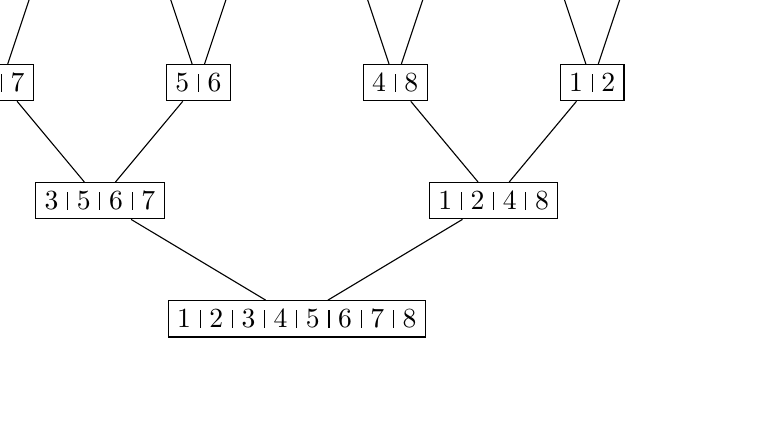
\begin{tikzpicture}
    \tikzstyle{every node}=[rectangle,draw]
    \tikzstyle{level 1}=[sibling distance=50mm]
    \tikzstyle{level 2}=[sibling distance=25mm]
    \tikzstyle{level 3}=[sibling distance=10mm]
    \node[rectangle,draw] {1 \vline \ 2 \vline \  3 \vline \  4 \vline
      \  5 \vline \  6 \vline \ 7 \vline \ 8} [grow'=up]
    child {node {3 \vline \ 5 \vline \  6 \vline \  7}
      child {node {3 \vline\ 7}
        child {node {3}}
        child {node {7}}
      }
      child {node {5 \vline\ 6}
        child {node {6}}
        child {node {5}}
      }
    }
    child {node {1 \vline \ 2 \vline \ 4 \vline \  8}
      child {node {4 \vline\ 8}
        child {node {8}}
        child {node {4}}
      }
      child {node {1 \vline\ 2}
        child {node {2}}
        child {node {1}}
      }
    }
    ;
  \end{tikzpicture}
\end{center}


\clearpage


\section{Matrix Multiplication}

\subsection{Divided into blocks of size $B$}

Suppose we are given an $N \times N$ matrix $A$, and another $N \times
N$ matrix $B$, and we are asked to find the product of the 2, we can
use the divide \& conquer algorithm to do so. We can split both
matrices into 4 parts and consider it to be a matrix multiplication of
two $4 \times 4$ matrices.

\[
Product =
\begin{pmatrix}
  a_{1,1} & a_{1,2} \\
  a_{2,1} & a_{2,2} 
\end{pmatrix}\times
\begin{pmatrix}
  b_{1,1} & b_{1,2} \\
  b_{2,1} & b_{2,2} 
 \end{pmatrix}
\]
\\
The number of multiplications needed for this is $8$.\\
\\
Now, if our matrix is stored such that when we reach a matrix of size
less than or equal to $\sqrt{B} \times \sqrt{B}$, we store that
complete matrix in one chunk rather than split the rows. If we store
the matrix in such a manner than multiplying two matrices with sizes
$\sqrt{B} \times \sqrt{B}$ each can be done using a constant number of
disk operations.\\
\\
This means that the number of matrices of size $\sqrt{B} \times
\sqrt{B}$ in the original matrix are $\frac{N}{\sqrt{B}}$. Hence, we get the
following recurrence for the number of multiplications required:\\
\\
$T(n) = 8T(\frac{n}{2}) + O(n^2)$\\
Substituting $n = \frac{N}{\sqrt{B}}$, we get the number of disk
transfers required:\\
$\Rightarrow T(n) = 8T(\frac{N}{2\sqrt{B}}) + O(\frac{N^2}{B})$\\
$\Rightarrow T(n) = \frac{N^3}{\sqrt{B}^3}$\\
$\Rightarrow T(n) = \frac{N^3}{{B}^{3/2}}$

\subsection{Divided into blocks of size $M$}

If we divide the matrix into blocks of size M (i.e. a matrix of size
$\sqrt{M} \times \sqrt{M}$, then we get $\frac{N}{\sqrt{M}}$ matrices
(or blocks) at the lowest level. Each such matrix can be read off from
the disk in time $O(\frac{M}{B})$.\\
\\
Hence, the recurrence for the number of disk transfers is:\\
$T(n) = \frac{M}{B} \times T'(n)$\\
$T'(n) = 8T(\frac{N}{2\sqrt{M}}) + O(\frac{N^2}{M})$\\
$\Rightarrow T(n) = \frac{M}{B} \times \frac{N^3}{M^{3/2}}$\\
$\Rightarrow T(n) = \frac{N^3}{B\sqrt{M}}$


\clearpage

\section{Matrix Multiplication}

\subsection{Recursion relation for the cost of a multiplication}

$T(n) = 8T(\frac{n}{2}) + O(n^2)$\\

\subsection{Number of memory transfers for divide \& conquer
  multiplication}

To compute the number of memory transfers for divide \& conquer
multiplication, we need to find out the number of memory transfers
required for multiplying 2 matrices of size $\sqrt{M} \times \sqrt{M}$
each (which is $\frac{M}{B}$) and multiply that by the number of
multiplications of matrices of size $\sqrt{M} \times \sqrt{M}$ needed
to multiply two matrices of size $N \times N$. This turns out to be:\\
\\
$T(n) = \frac{M}{B} \times T'(n)$\\
$T'(n) = 8T(\frac{N}{2\sqrt{M}}) + O(\frac{N^2}{M})$\\
$\Rightarrow T(n) = \frac{M}{B} \times \frac{N^3}{M^{3/2}}$\\
$\Rightarrow T(n) = \frac{N^3}{B\sqrt{M}}$


\clearpage

% van Emde Boas problems
\section{Deletions in vEB Tree}
Find the predecessor and successor of the element to be deleted. Let us call them $p$, $s$,
and $e$ respectively. 

Now traverse down the path of the vEB tree with $e$ as the index. If $p$ and $s$ belong to the
same widget, then just recusively delete the element $e$ from the child widget. If $p$ does not
belong to the current widget, but $s$ does, set the min of the current widget to $s$. If $s$ does
not belong to the current widget, but $p$ does, set the max of the current widget to $p$. If 
neither of them exist, then mark the min and max of the current widget as -$\infty$ and +$\infty$
respectively, and recurse. 
(TODO: Verify)

\clearpage

\section{vEB Tree in $O(n)$ space}
The naive version of vEB tree takes $O(u)$ space. However, this is wasteful since, not all
the widgets would be in use at the very same time. From the Hashing lecture in class, we 
know that we can hash $n$ elements in $O(n)$ space, while having an $O(1)$ query time 
(TODO: Revise the Hashing lecture).

Now, instead of explicitly maintaining, we create widgets and allocate space for them
dynamically. We create a hash-table on the widget index, and set the key as the location in
memory where we have allocated space for the widget. 

(TODO: How do we prove that inserting $O(n)$ widgets would use up only $O(n)$ space? I have 
a rough idea, nothing formal)

Now, instead of indexing into the array as we did earlier for a widget, we now lookup in the 
hash-table to find the location where we have stored the widget, and inspect the widget at that 
location, and proceed appropriately. The rest of the algorithm remains the same.


\end{document}
